\documentclass[12pt]{article}

\usepackage{titling}
\usepackage{tikz}
\usepackage{fancyhdr}
\usepackage[utf8]{inputenc}
\usepackage{amsmath}
\usepackage[affil-it]{authblk}
\usepackage{graphicx}
\usepackage[
    backend=biber,
    style=ieee,
    citestyle=authoryear,
    sortlocale=dk_DK,
    language=danish,
    urldate=long,
    sorting=nty,
]{biblatex}
\addbibresource{bib.bib}
\usepackage[]{hyperref}

\renewcommand*\contentsname{Indholdsfortegnelse}

%%%%%%%%%%%%%%%%%%%%%%%%%%%%%%%%%%%%%%%%%%%%%%%%%%%%%%%%%%%%%%%%%%%%%%%%%%%%

\title{3g SRP - Kunstig intellegens}
\author{Jeppe Møldrup}
\affil{Nørresundby gymnasium og HF}
\date{21/12-2018}

%%%%%%%%%%%%%%%%%%%%%%%%%%%%%%%%%%%%%%%%%%%%%%%%%%%%%%%%%%%%%%%%%%%%%%%%%%%%

\begin{document}
\begin{titlingpage}
\clearpage\maketitle
\thispagestyle{empty}
\noindent\rule{\textwidth}{0.4pt}\\
\\

\includegraphics[width=\textwidth]{pic/logo.png}
\noindent\rule{\textwidth}{0.4pt}
\pagebreak

\begin{abstract}
        abstract
\end{abstract}

\end{titlingpage}
\pagebreak

\tableofcontents
\pagebreak

\section{Redegørelse af et ANN netværk}

\subsection{ANN's baggrund}
Et ANN(Artificial Neural Network) er en form for kunstig intellegens, hvor man prøver at efterligne den menneskelige hjerne
ved at lave simple versioner af det netværk af de mange milliarder neuroner der findes i den menneskelige hjerne.
Ligesom hvor en biologisk menneskehjerne har neuroner og synapser med forskellige styrker, så har et ANN også det, dog lidt simplere
så man kan tillægge værdier til de forskellige neuroner og synapser.

\subsection{Strukturen bag et ANN}
I den menneskellige hjerne er der som sagt milliarder af forskellige neuroner \footcite{DDOhjerne}.
I et ANN laver man ikke ligeså mange
neuroner som i en rigtig hjerne, da det er umuligt med den teknologi vi har i dag, men det er stadigvæk i fokus at lave et netværk med så mange neuroner
som muligt.
Derfor er det vigtigt at disse neuroner er matematisk set meget simple, så det er nemt for en moderne computer bare at blæse gennem matematikken
i et ANN. Så den strukter man så har valgt bag én neuron i et givet ANN er figur 1.

\begin{figure}
\label{neuron}
\caption{Model af en neuron}
\LARGE
\begin{center}
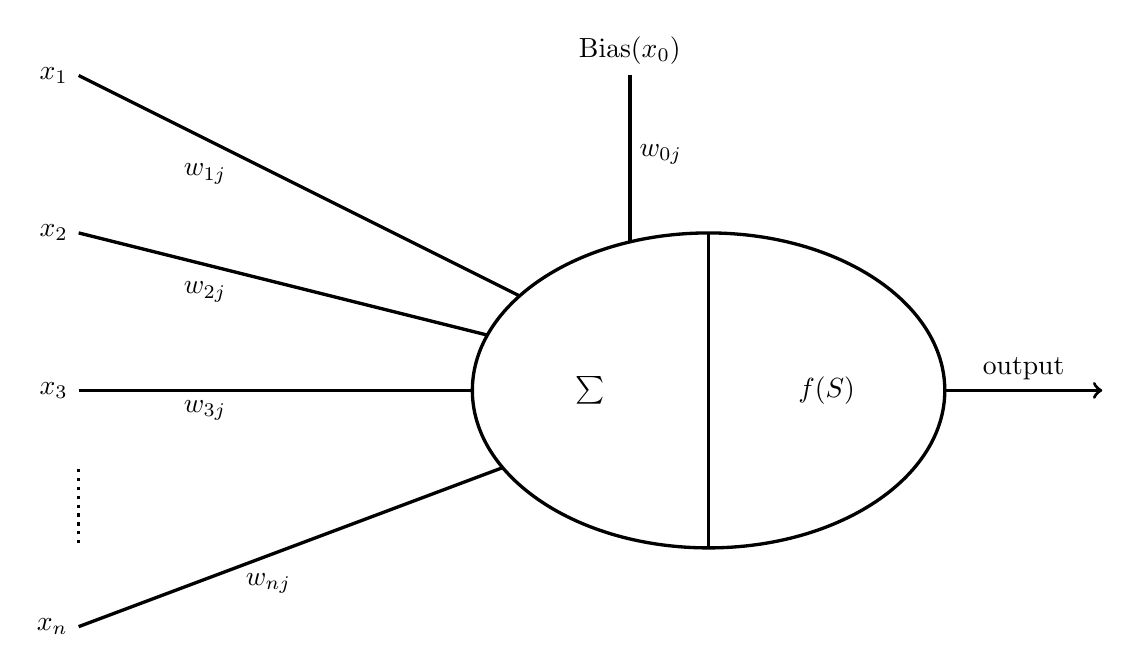
\begin{tikzpicture}

        \draw[very thick] (-1, 4) node[anchor=south]{Bias($x_0$)} -- (-1, 0);
        \draw[very thick] (-8, 4) node[anchor=east]{$x_1$} -- (0, 0);
        \draw[very thick] (-8, 2) node[anchor=east]{$x_2$} -- (0, 0);
        \draw[very thick] (-8, 0) node[anchor=east]{$x_3$} -- (0, 0);
        \draw[very thick, dotted] (-8, -1) -- (-8, -2);
        \draw[very thick] (-8, -3) node[anchor=east]{$x_n$}-- (0, 0);

        \node[anchor=west] at (-1, 3){$w_{0j}$};
        \node[anchor=north east] at (-6, 3){$w_{1j}$};
        \node[anchor=north east] at (-6, 1.5){$w_{2j}$};
        \node[anchor=north east] at (-6, 0){$w_{3j}$};
        \node[anchor=north west] at (-6, -2.2){$w_{nj}$};

        \draw[very thick, fill=white] (0, 0) ellipse (3 and 2);
        \draw[very thick] (0, 2) -- (0, -2);
        
        \node at (-1.5, 0){$\sum$};
        \node at (1.5, 0){$f(S)$};

        \draw[very thick, ->] (3, 0) -- (4, 0) node[anchor=south]{output} -- (5, 0);

\end{tikzpicture}
\end{center}
\normalsize

\end{figure}

Hvor alle $x_n$ er outputs fra andre neuroner der er tilsluttet denne neuron via synapser, $w_{nj}$ er såkaldte vægte der angiver hvor
forstærket signalet er fra outputtet af sidste neuron og bias er en værdi der der enten vil øge eller
sænke outputtet af en given neuron. Det der så sker inde i neuronen er to ting. \\
Først bliver alle inputs ganget sammen med deres vægte og summeret op. \\
Derefter bliver der ført en såkaldt "Activation function" der typisk bare normaliserer
summationen mellem f.eks 0 og 1\footcite{ANN11}. Her betragter jeg bare logistisk vækst med et maksimum på 1 som min activation function.
Funktionen vil så tage et vilkårligt tal og så spytte et andet tal ud der ligger mellem 0 og 1
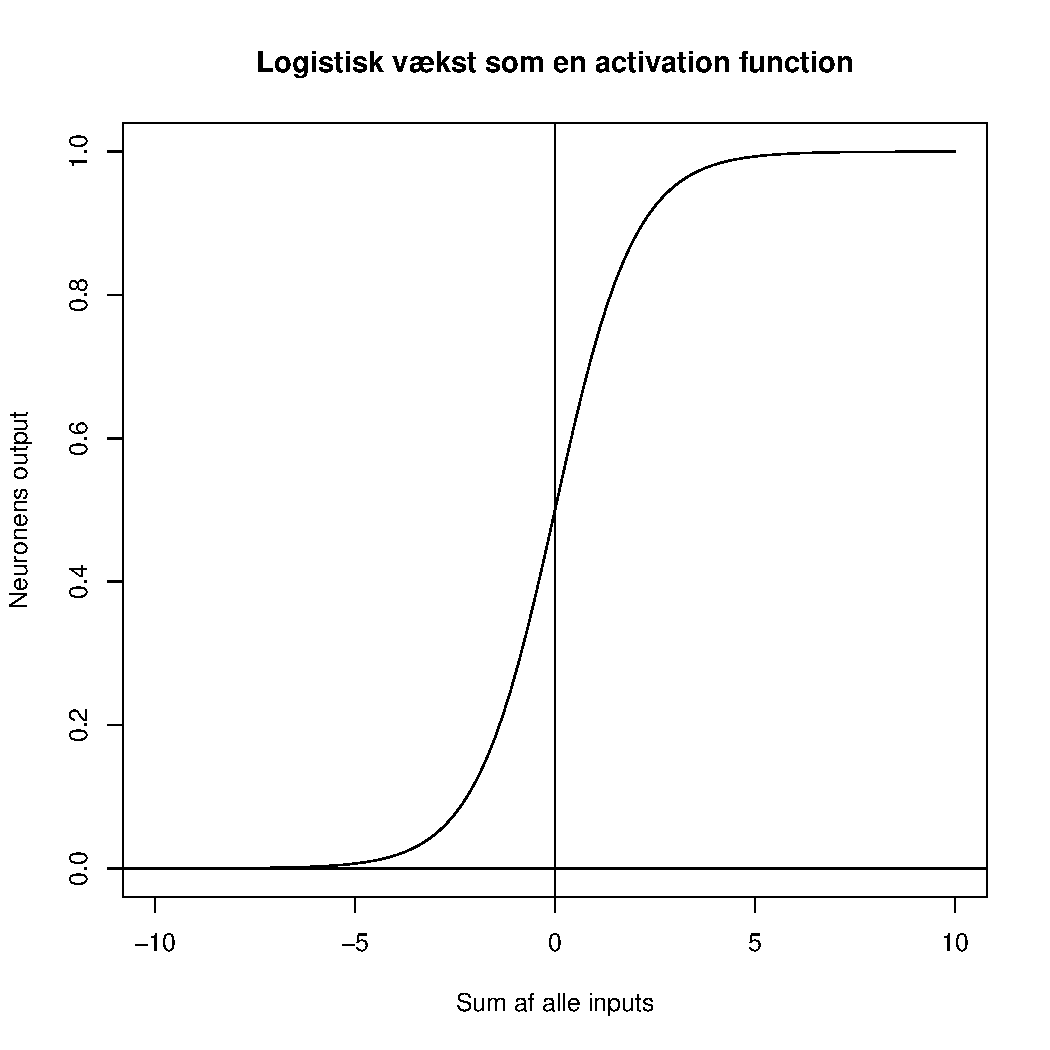
\includegraphics[width=\textwidth]{diagrammer/sigmoid.pdf}

Så det er strukturen bag én enkelt neuron. Netværket består af en hel masse neuroner der er sammensat således

\begin{figure}
\label{netvaerk}
\caption{Model af et neuralt netværk}
\LARGE
\begin{center}
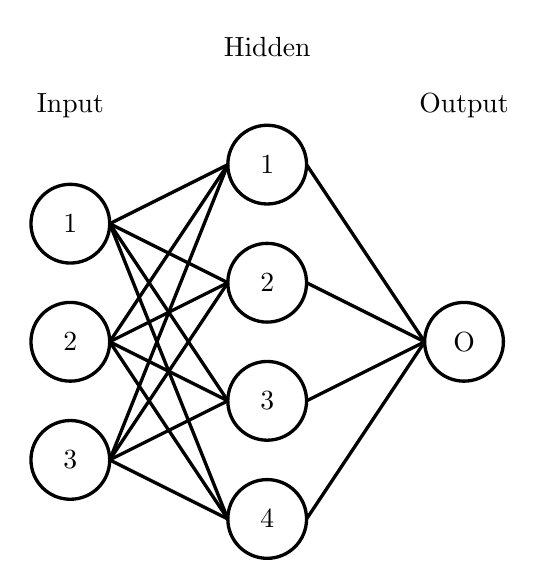
\begin{tikzpicture}

        \foreach \x in {1, 2, 3}
        {
                \draw[very thick] (0, -1.5*\x) circle (0.5);
                \node at (0, -1.5*\x) {\x};
                \foreach \y in {1, 2, 3, 4}
                {
                        \draw[very thick] (0.5, -1.5*\x) -- (2, -1.5*\y+0.75);
                }
        }

        \foreach \y in {1, 2, 3, 4}
        {
                \draw[very thick] (2.5, -1.5*\y+0.75) circle (0.5);
                \node at (2.5, -1.5*\y+0.75){\y};
                \draw[very thick] (3, -1.5*\y+0.75) -- (4.5, -3);
        }
        \draw[very thick] (5, -3) circle (0.5);
        \node at (5, -3){O};
        
        \node at (0, 0){Input};
        \node at (2.5, 0.75){Hidden};
        \node at (5, 0){Output};

\end{tikzpicture}
\end{center}
\normalsize

\end{figure}

Figur 2 er et eksempel på et meget simpelt netværk der er kendt som et Feed Forward Artificial Neural Network, eller FFANN.
Her bliver alle neuroner delt op i forskellige lag, i det her eksempel er der 3, men der kunne også være flere. Det første lag
kaldes for "Input layer", det sidste kaldes for "Output layer" og alle imellem kaldes for "Hidden layers". Så er inputtet
til hver neuron outputtet fra alle neuroner i sidste lag. Grunden til at alle neuroner i et givent lag så ikke har den samme værdi
idet deres værdi afhænger af samme neuroner, er fordi de alle sammen har forskellige vægte. Så f.eks. har første neuron 4 forskellige vægte,
én til hver af neuronerne i næste lag\footcite{ANN11}. Allerede i dette meget simple netværk er der ret rodet i forhold til de små tilslutninger mellem neuronerne.
Så derfor er det smart at have en god systematisk navngivning til de forskellige elementer der opgør et neuralt netværk.\\
Følgende navngivning vil blive brugt.\\
Neuroner(Hvor indexet 0 betyder bias:\\
Input: $I_{i}$~~~~Hidden: $H_{i}$~~~~Output: $O_{i}$ \\
Vægte har i indekset 2 numre, et nummer for hvilken neuron de er fra, og et nummer for hvilken neuron de skal til, derudover også  en indeks der viser hvilket lag de er fra
$w_{ij}^{l}$, så det kunne f.eks. være $w_{11}^I$, hvor vægten er fra input laget, og den går fra første neuron til første neuron af hidden laget(Igen er indekset 0 vægten til
biasset).

\section{Fremstilling af robotter i Isaac Asimov: "Robot"}
Isaac Asimov's fortællinger i novellesamlingen "Robot" finder sted i samme univers og deler karakterer mellem hinanden, bogen handler nemlig om
robotpsykologen Dr. Susan Calvin der har en samtale med en journalist fra avisen "Interplanetary Press", hvor hun så fortæller om nogle forskellige episoder eller
vanskeligheder hun har oplevet gennem sin karriere i robot-industrien.
\\
\\
Isaac Asimov har til denne bog lavet tre love som han mener er tilstrækkelige for at kunne lave sikre robotter der adlyder mennesker, lovene lyder:
\begin{enumerate}
\item[1.] En robot må ikke skade noget menneske eller, ved at undlade at handle, tillade at et menneske bliver skadet.
\item[2.] En robot skal adlyde de ordrer, et menneske giver den, undtagen hvor disse ordrer ville stride mod den første lov.
\item[3.] En robot skal opretholde sin egen eksistens, medmindre denne selvopholdelse er i modstrid med den første eller den anden lov.\footcite[7]{robot}
\end{enumerate}

De forskellige histiorier har nogenlunde det samme tema, hvor der er et eller problem med en robot, den opfører sig ikke som den skal, og så skal de ud fra
robotikkens tre love finde ud af hvorfor robotten opfører sig sådan, og hvordan de kan fikse det så den gør hvad de vil.
\\
\\
Selve robotterne bliver overvejene fremstillet på en positiv måde i teksterne, dette kan ses f.eks. i citatet \textit{"Men sagen er den, at man simpelthen
ikke kan skelne mellem en robot og de allerbedste mennesker"}\footcite[194, l. 5]{robot}, men robotterne bliver i teksterne stadig handlet med respekt,
som det sis i citatet \textit{"Fysisk set og i en vis forstand psykisk set er en robot, enhver robot, menneskene overlegen. Hvad gør dem så til slaver?
Kun den første lov! Ja, uden den ville den første ordre, du prøvede på at give en robot, føre til, at du blev slået ihjel."}\footcite[130, l. 31]{robot} som
er fra en historie i bogen hvori de har nogle robotter der ikke har hele den første lov "imprentet" i hjernen.

\subsection{Rundt i ring}

Problemet eller konflikten der opstår i teksten "Rundt i ring" er hvor de har en robot ved navn "Speedy" som var blevet sendt ud på solsiden af merkur,
hvor der var en sø af selen som den skulle hen for at indsamle, men Speedy kommer af en eller anden grund ikke tilbage. Da de kiggede på hans position viste det sig
at Speedy bare løb rundt i en cirkel rundt om søen. Speedy er en særlig dyr model og derfor er dens tredje lov forstærket, dvs. den har en stor modvilje mod
fare, og i nogle tilfælde med en ekstrem stor fare ville det kunne overdøve den anden lov, hvis ordreren ikke var givet med noget særligt tryk der gjorde den
ekstra vigtig. Og dette var lige det der skete med speedy. De to videnskabsmænd Mike Donovan og Gregory Powell fandt frem til at der måtte være en særlig fare der befandt
sig i midten af søen, som når den var langt væk var det ordreren om at hente selen der var stærkest, men hvis den kom tæt nok på var det speedy selvopholdelse
der var stærkest, det resulterede i at robotten bare blev ved et punkt hvor de var lige store og løb rundt i cirkel rundt om søen. Så for at få speedy til at komme tilbage igen
skulle Mike og Gregory gøre noget der ville overdøve både den tredje og den anden lov, og det eneste der overdøver begge to er den først lov. Så de var nødt til at sætte
sig selv i fare, så speedy ville komme tilbage til sine sanser og komme og rede dem, og derved opretholde den første lov. Den måde de gjorde det på var at Gregory gik ud i solen
hvor han som menneske ikke kunne overleve særlig længe, og på den måde kom speedy atter tilbage da den første lov negerer de to andre, og redede ham fra at dø.
\\
\\
Her bliver robotten speedy fremstillet som om den ikke virker i starten, men til sidst finder man så ud af at grunden til at den opførte sig så besynderligt var pga. en menneskefejl idet
den ordrer den fik ikke var præcis og fokuseret nok på hvor vigtigt det var for speedy at indsamle selenen. Og derfor kom der et uventet resultet fra robotten, nemlig det at den cirklede
rundt om søen i stedet for at indsamle selenen.

\subsection{Logik}

I \textit{Logik} står Mike og Gregory med en eksperimentel robot der hedder Emsig. Problemet med Emsig er at han er en skeptiker, og f.eks. ikke tror på at Mike og Gregory
har samlet ham, men i stedet vil han gennemtænke ting logisk. Efter nogle dage kom Emsig til den logiske konklusion at det ikke var muligt for menneskene at lave et væsen
der er dem selv overlegent, og derfor måtte det være et væsen der er mægtigere end Emsig, nemlig herren. Derudover før Emsig nogle robot tilhængere og nærmest skaber
en hel kult af robotter der tjener \textit{Herren}. Men det viser sig at selv om Emsig næsten driver de to mænd til vanvid med sin snak om herren og logik, så virker
Emsig alligevel som han burde, nemlig til at holde styr på apparaterne ved stationen.
\\
\\
I denne tekst bliver der draget ligheder mellem robotterne og mennesker, ved f.eks. at Emsig er overbevist om at han og alle andre er skabt af \textit{Herren}.
Og især med Emsig's citat \textit{"Jeg har koncentreret mig om mine egne tanker de to sidste dage, sagde Emsig, og resultaterne har været overordentlig
interessante. Jeg begyndte med den ene sikre præmis, jeg følte mig berettiget til at komme med. Jeg eksisterer selv, fordi jeg tænker"}\footcite[62, l. 25]{robot} hvor Asimov nærmest
gør grin med René Descartes meget berømte udsagn \textit{"Cogito, ergo sum"}\footcite{rene}, som betyder det samme. Så denne tekst viser hvordan en robots hjerne er meget ligesom et menneskes og derfor
hvis en robot lades være alene med sine egne tanker vil den udvikle mange af de samme ting som mennesker har udviklet, dvs. religioner, philosofiske tanker osv.

\subsection{Bevis}

\textit{Bevis} finder sted ikke så lang tid før et valg, hvor der er to primære kandidater, Stephen Byerley og Francis Quinn. Quinn kommer til Lanning, der ejer United States Robots and Mechanical Men,
med den påstand at hans modkandidat Byerley er en robot. Quinns årsag er fordi at man aldrig ser Byerley spise, sove eller drikke noget. Efter at gå frem og tilbage lidt finder de ud af
at de hverken kan bevise eller modbevise påstanden om at Byerley er en robot. Indtil under en offentlig tale fra Byerley, kommer der en person op på scenen og beder Byerley om at slå ham. Hvis han
er en robot ville han ikke kunne dette da det går imod robotikkens første lov, men til folks overraskelse, så slår Byerley ham rent faktisk. Dog har Calvin i tankerne at hvis personen som kom op
på scenen faktisk ikke var en person, men også en robot som var med på den. Ville Byerley godt kunne slå vedkommene selv hvis han var en robot, idet det ikke strider imod første lov. Så i
historien får de hverken modbevist eller bevist at Byerley er en robot, med der bliver vist hvor vigtig robotikkens love er.
\\
\\
Det er også fra denne tekst citatet \textit{"Men sagen er den, at man simpelthen ikke kan skelne mellem en robot og de allerbedste mennesker"}\footcite[194, l. 5]{robot} som jeg brugte
før kommer fra. Idet dilemmaet er at enten er Byerley en robot, eller så er han et meget godt menneske.

\subsection{Konklusion på Isaac Asimov: "Robot"}

Alt i alt bliver robotterne fremstillet positivt, som noget der sammen med mennesker kan skabe en lysere fremtid, men selvfølgelig ikke uden nogle bump. Derudover bliver
de tre love indenfor robotikken fremstillet som værende meget vigtig, og at der ikke kan eller burde skabes nogle former for robotter der ikke har disse tre love brændt
dybt ned i hjernen. Idet som Calvin selv siger, det eneste der holder robotterne under kontrol af menneskene er disse tre love, uden dem er der ingen net der
holder robotterne fra at indtage deres retmæssige plads i toppen af fødekæden og enten udryde mennesker eller gøre dem til slaver.

\section{Asimovs tre love i forhold til ANN}

Hvis vi forestiller os en hypotetisk fremtid der minder lidt om Isaac Asimovs univers i Robot, hvor der finder fysiske robotter styret af en form for kunstig intellegens
der gør dem bevidste, kunne man forestille sig at hvis ikke der var implementeret en form for arbejdsetik dybt i deres hjerner der gør at de adlyder mennesker, at de måske ikke
ville gøre som vi siger idet vi ikke rigtig kan tvinge dem. Da ANN er en form for kunstig intellegens der er baseret på en simpel model af den menneskelige hjerne, kunne man
nok godt forestille sig at disse robotter vil have et ANN som deres hjerne. Hvis vi så ignorerer selve det tekniske ved implementationen af de tre robotlove i et ANN, så kunne
man forestille sig at de nok ville være tilstrækkelig til at holde en kunstil intellegens under kontrol. Problemet ligger i at kunne implemeterer robotlovene ordentligt så det
er umuligt for en robot at overtræde dem. Hvis et ANN der f.eks. var beregnet til at fjerne spam-emails og ikke havde de tre love indført, så ville den måske tage det logiske
skridt og fjerne alle mennesker idet alt spam er et resultat af mennesker, og hvis man bare gjorde den menneskelige race uddød så vil man også fjerne alt spam. Det lyder måske
ret urealistisk, men det er det faktisk ikke, fordi et ANN tænker ikke ligesom et menneske, et ANN finder bare den mest eller tæt på den mest effektive løsning på et problem. Og
hvis den mest effektive måde at løse et problem på er ved at fjerne alle mennesker, så er det sådan et ANN vil løse det på. Et ANN har ikke nogen form for sympati eller empati,
det er derfor man tager de etiske spørgsmål i forhold til kunstig intellegens så seriøst.

\subsection{Københavns Universitet}

Diskussionen om etiske regler bag kunstig intellegens er f.eks. blevet taget op af Københavns Universitet, hvor professor Peter Sandøe og lektor Sune Hannibal Holm,
vil bruge de næste to års tid på at diskutere med alle forskellige politiske og samfundsmæssige synspunkter hvordan man skal arbejde med kunstig intellegens sikkert,
og flette hele den diskussion sammen til en form for etisk kodeks. De forskellige etiske spørgsmål de vil kigge på er f.eks. hvem der har skylden
når en selvkørende bil kører galt, om politiet må bruge kunstig intellegens som et hjælpemiddel til at forudsige, hvem der begår kriminalitet osv.\footcite{kunyt} Dilemmaet med den
selvkørende bil lyder for mange som et vi nok kommer ud for om nogle år når vi engang får selvkørende biler på vejene. Men tværtimod så er det et dilemma som vi faktisk allerede er
kommet ud for tidligere i år den 18. marts 2018, hvor en selvkørende bil fra uber påkørte en dame i Arizona, USA og dræbte hende.\footcite{nyt}, så det er ikke bare nok at gøre
alt hvad vi kan for at gøre disse systemer baseret på kunstig intellegens så sikre som muligt. Men vi er også nødt til at udvikle en hel ny kodeks der siger hvem der er skyld
i vilke ulykker når disse systemer tager fejl.

\subsection{Robotters rettigheder og fri vilje}

I Isaac Asimovs bog Robot, bliver robotterne fremstillet som nogle meget højteknologiske redskaber som mennesker har udviklet. Så som en form for slaver der arbejder for mennesker.
Men Singularitets-instituttet for Kunstig Intellegens mener man bør skelne mellem kunstig intellegens med og uden bevidsthed. Og at man skal begynde måske endda at snakke om
robot rettigheder for kunstig intellegens med "ægte bevidsthed", idet Asimovs robotlove begrænser robotternes frie vilje og degraderer robotter til menneskenes slaver. Så der er
nogle der mener at man ikke burde indprente Asimovs love ind i en bevidst kunstig intellegens og derfor vil indføre en række rettigheder til robotter der minder lidt om
menneske- og dyrerettigheder. Problemet med de kunstige intellegenser der er bevidste bliver så at hvis de får rettigheder kan det tage væk fra hvad de egentlig var udviklet til,
nemlig at hjælpe mennesker. Men hvis ikke man giver dem rettigheder kan det minde om slaveri og plageri idet robotterne rent faktisk er bevidste.\footcite{etikr}\footcite{robri}
\\
\\
Så alt i alt er de etiske spørgsmål der kommer med kunstig intellegens en politisk glidebane, hvori en forkert beslutning kan resultere i menneskenes undergang, eller en helt
ny episode i historiebøgerne om slaveri.


\printbibliography[type=book, title={Referencer \\ Bøger}]
\printbibliography[type=online, title={Artikler og andre online kilder}]
\end{document}
